\onlyinsubfile{\setcounter{section}{6}}
\section{Extension: Estimating a Lognormal distribution of returns}
\notinsubfile{\label{sec:lognorm}}

\par As I mentioned before, \cite{aflgdmlp20} document a persistent component to individual returns using the Norwegian population data. In fact, they include a graphic of the distribution of the estimated fixed effect in the return to net worth for individuals, which is clearly not uniformly distributed. For this reason, I rerun the estimation of my model under the assumption that returns are instead lognormally distributed across households. As we will see, the takeaways from my paper are robust to this change.

\subsubsection{Comparing the simulated wealth distributions}

\par Since the model without heterogeneous returns is the same regardless of the distributional assumptions, below I include a figure of the results for the infinite horizon and life cycle models with heterogeneous returns, lognormally distributed across households. 

\begin{figure}[h]
    \centering
    \begin{minipage}{0.48\textwidth}
        \centering
        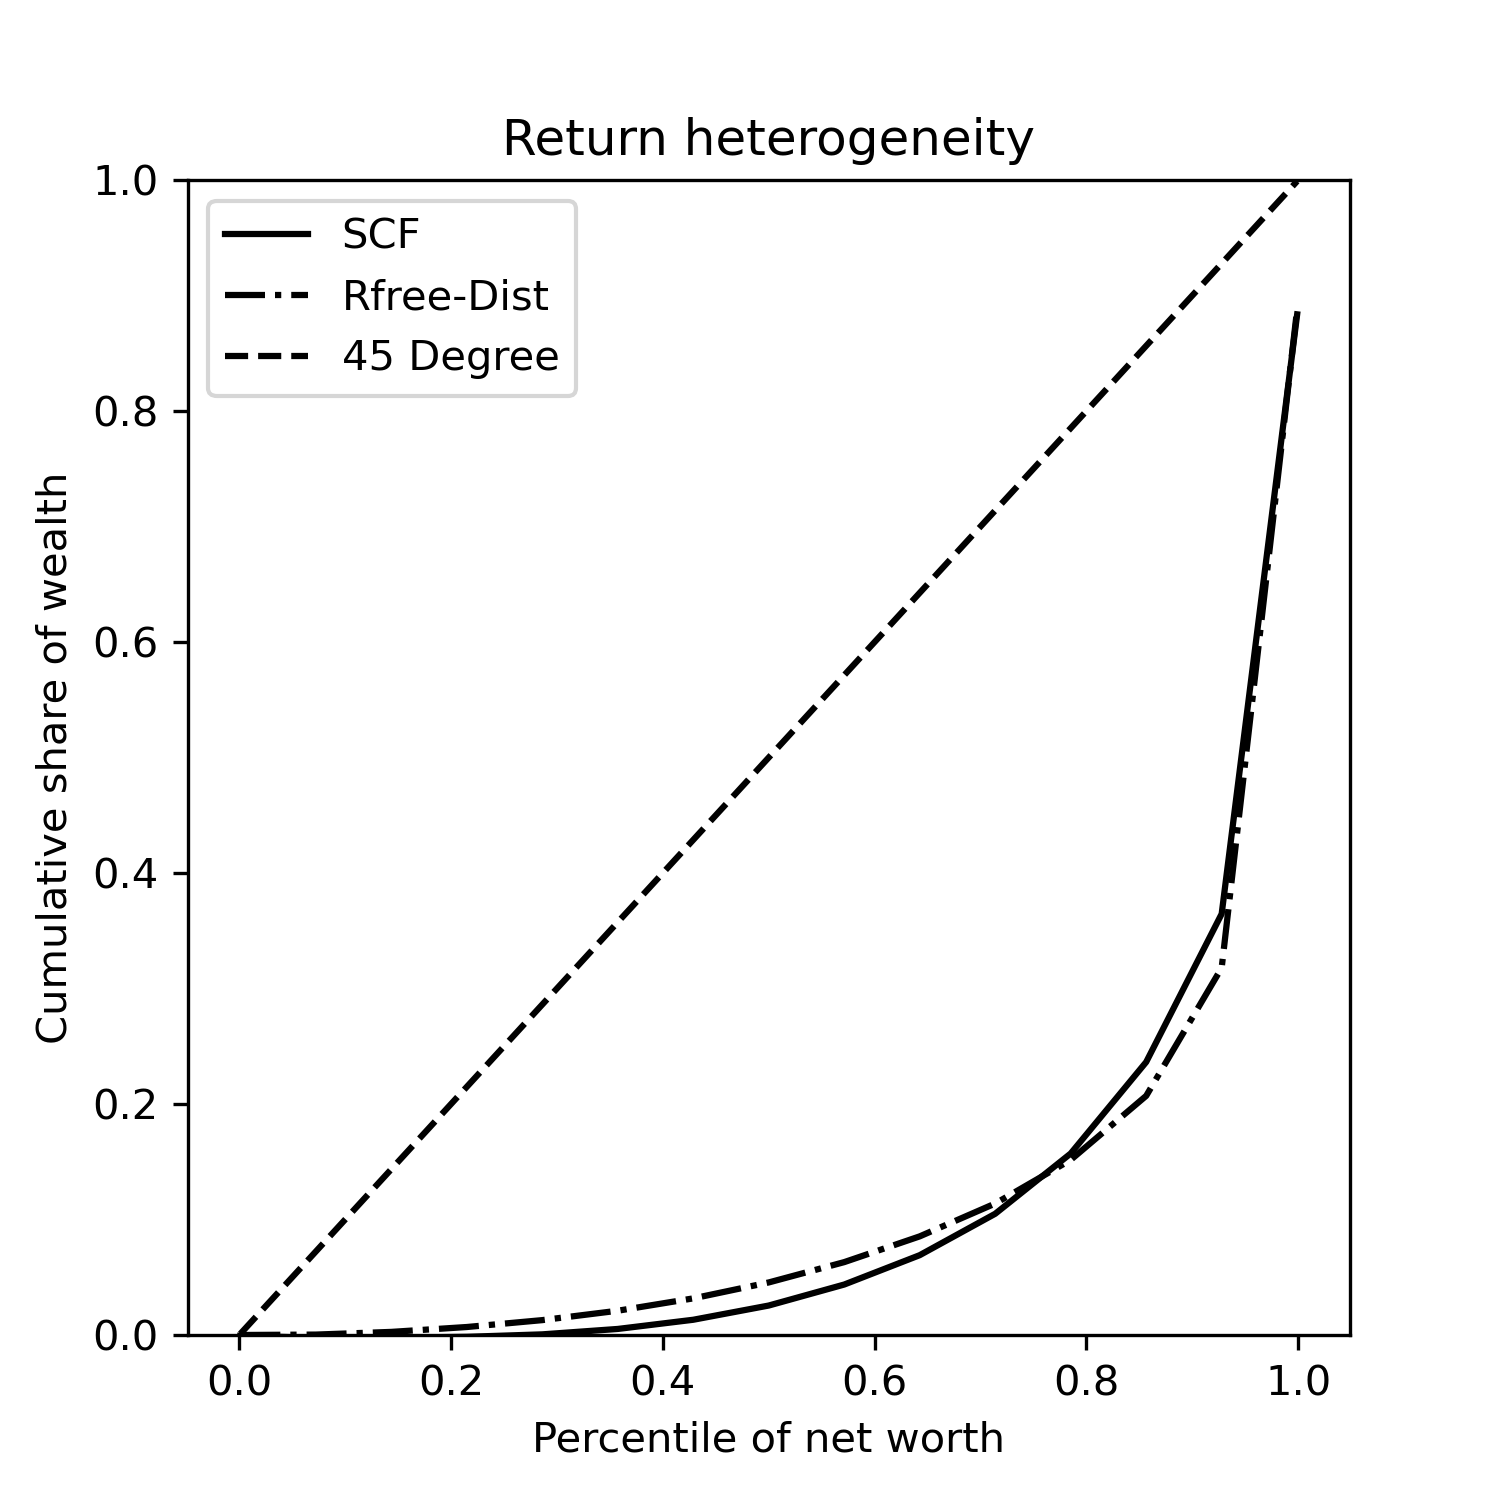
\includegraphics[width=\textwidth]{../Figures/Lognorm_PYrrDistNetWorth_2004Plot.png}
    \end{minipage}
    \hfill
    \begin{minipage}{0.48\textwidth}
        \centering
        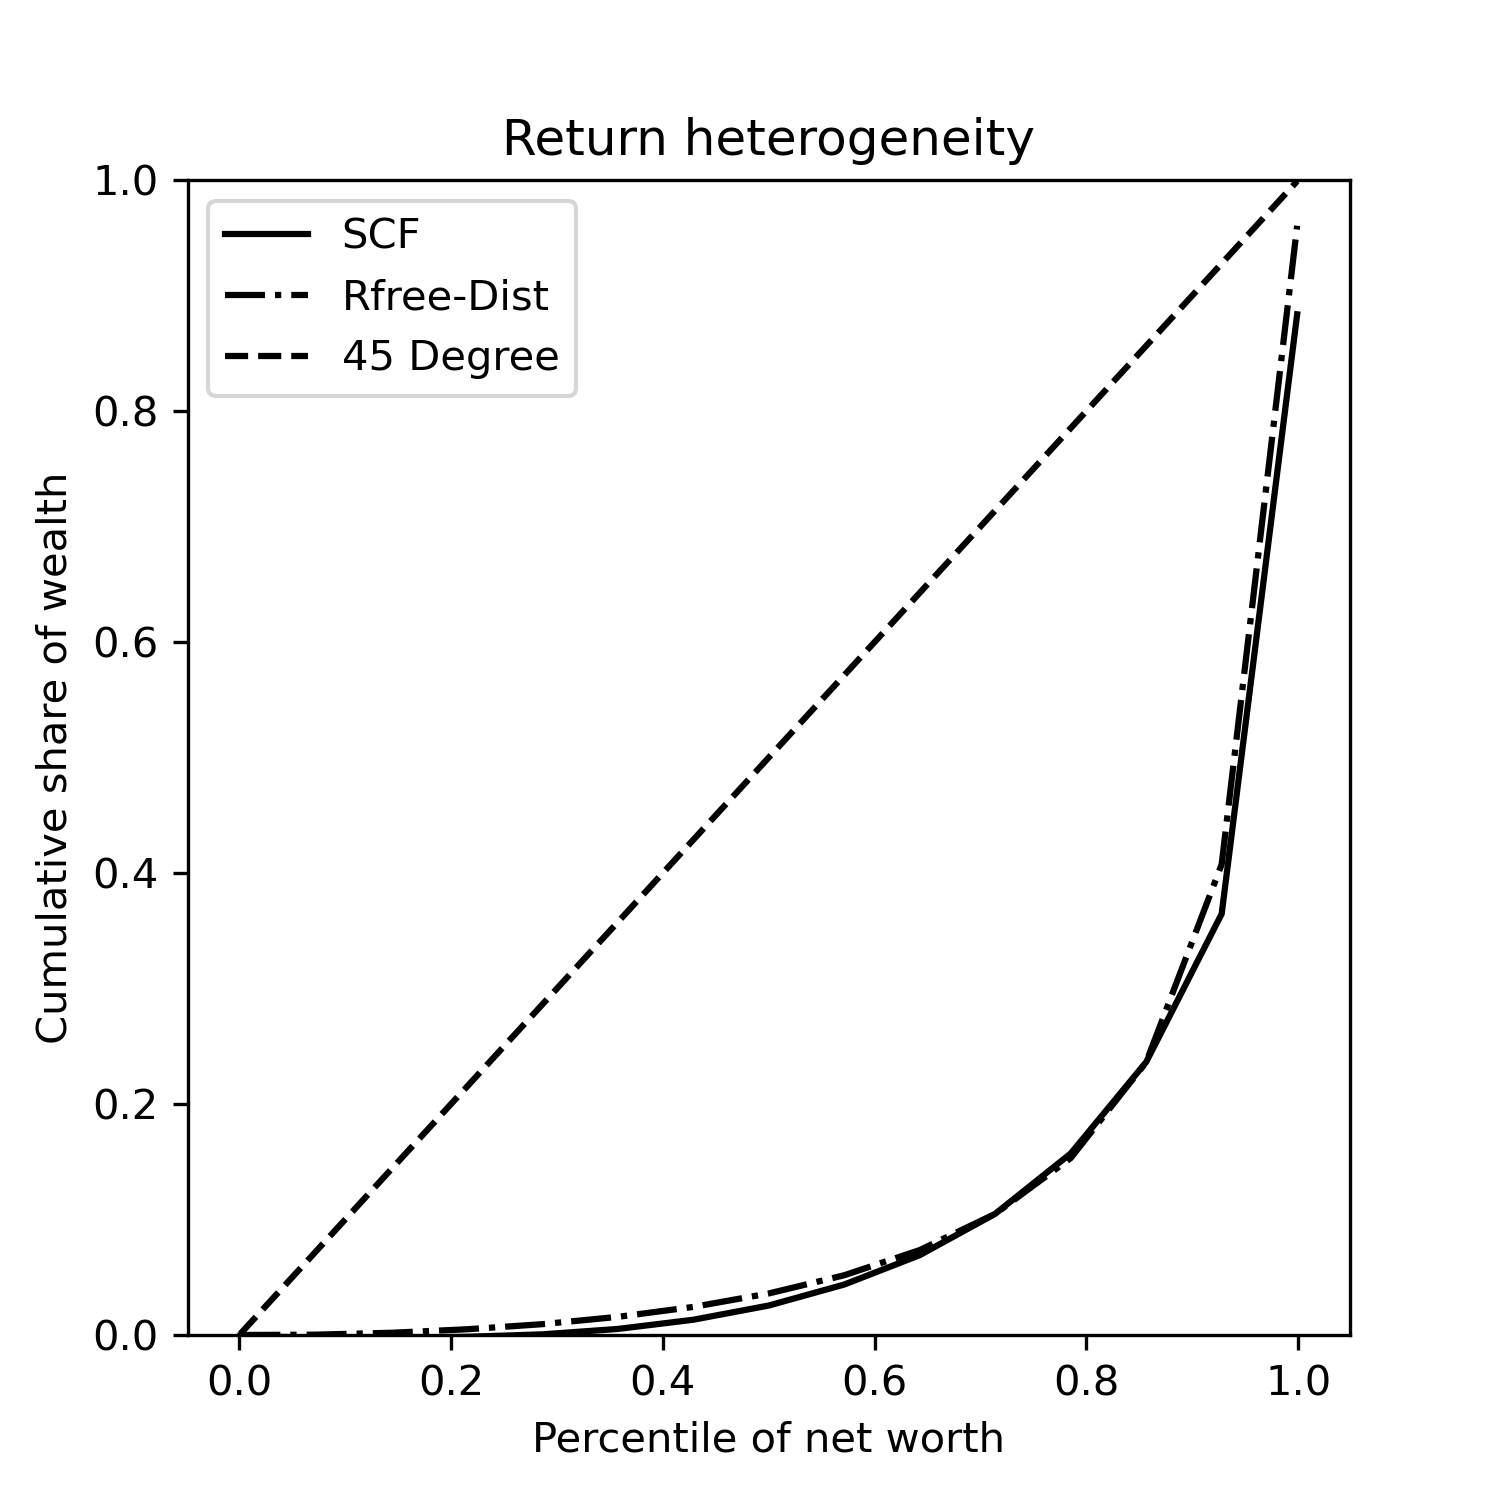
\includegraphics[width=\textwidth]{../Figures/Lognorm_LCrrDistNetWorth_2004Plot.png}
    \end{minipage}
    \caption{Comparison of PY (left) vs LC (right) R-Dist Models.}
    \label{fig:PYLCLognorm} 
\end{figure}

\par It is clear from the figure that the same pattern appears here: the life cycle setting is better at matching the observed wealth distribution than the infinite horizon setting, but they both match wealth moments especially well. Again, I include the table of those wealth moments for each of the models and the data below. 

\begin{table}[htbp]
\centering
\caption{Wealth Distribution (Lognormal Returns)}
\label{tab:Lognorm_PY_LC_wealth_distribution_compare}
\small
\setlength{\tabcolsep}{10pt}
\renewcommand{\arraystretch}{1.15}
\resizebox{\textwidth}{!} \\
\hline
\textbf{Wealth share (data)} & -0.002 & 0.011 & 0.044 & 0.118 & 0.255 & 0.574 \\
\textbf{Wealth share (PY)}   &  0.006 & 0.021 & 0.044 & 0.088 & 0.225 & 0.616 \\
\textbf{Wealth share (LC)}   &  0.004 & 0.016 & 0.039 & 0.107 & 0.335 & 0.498 \\
\hline\hline
\end{tabular}%
}
\end{table}



\subsection{Untargeted moments}

\par In the infinite horizon case, the aggregate MPC is $25.7\%$. The aggregate MPC in the life-cycle setting is essentially the same: $26\%$. Below is the breakdown of average MPCs by wealth deciles for both settings. Again, the MPC's are higher in general in the life-cycle setting since it is able to match lower moments of the wealth distribution better. 

\begin{figure}[htbp]
\centering
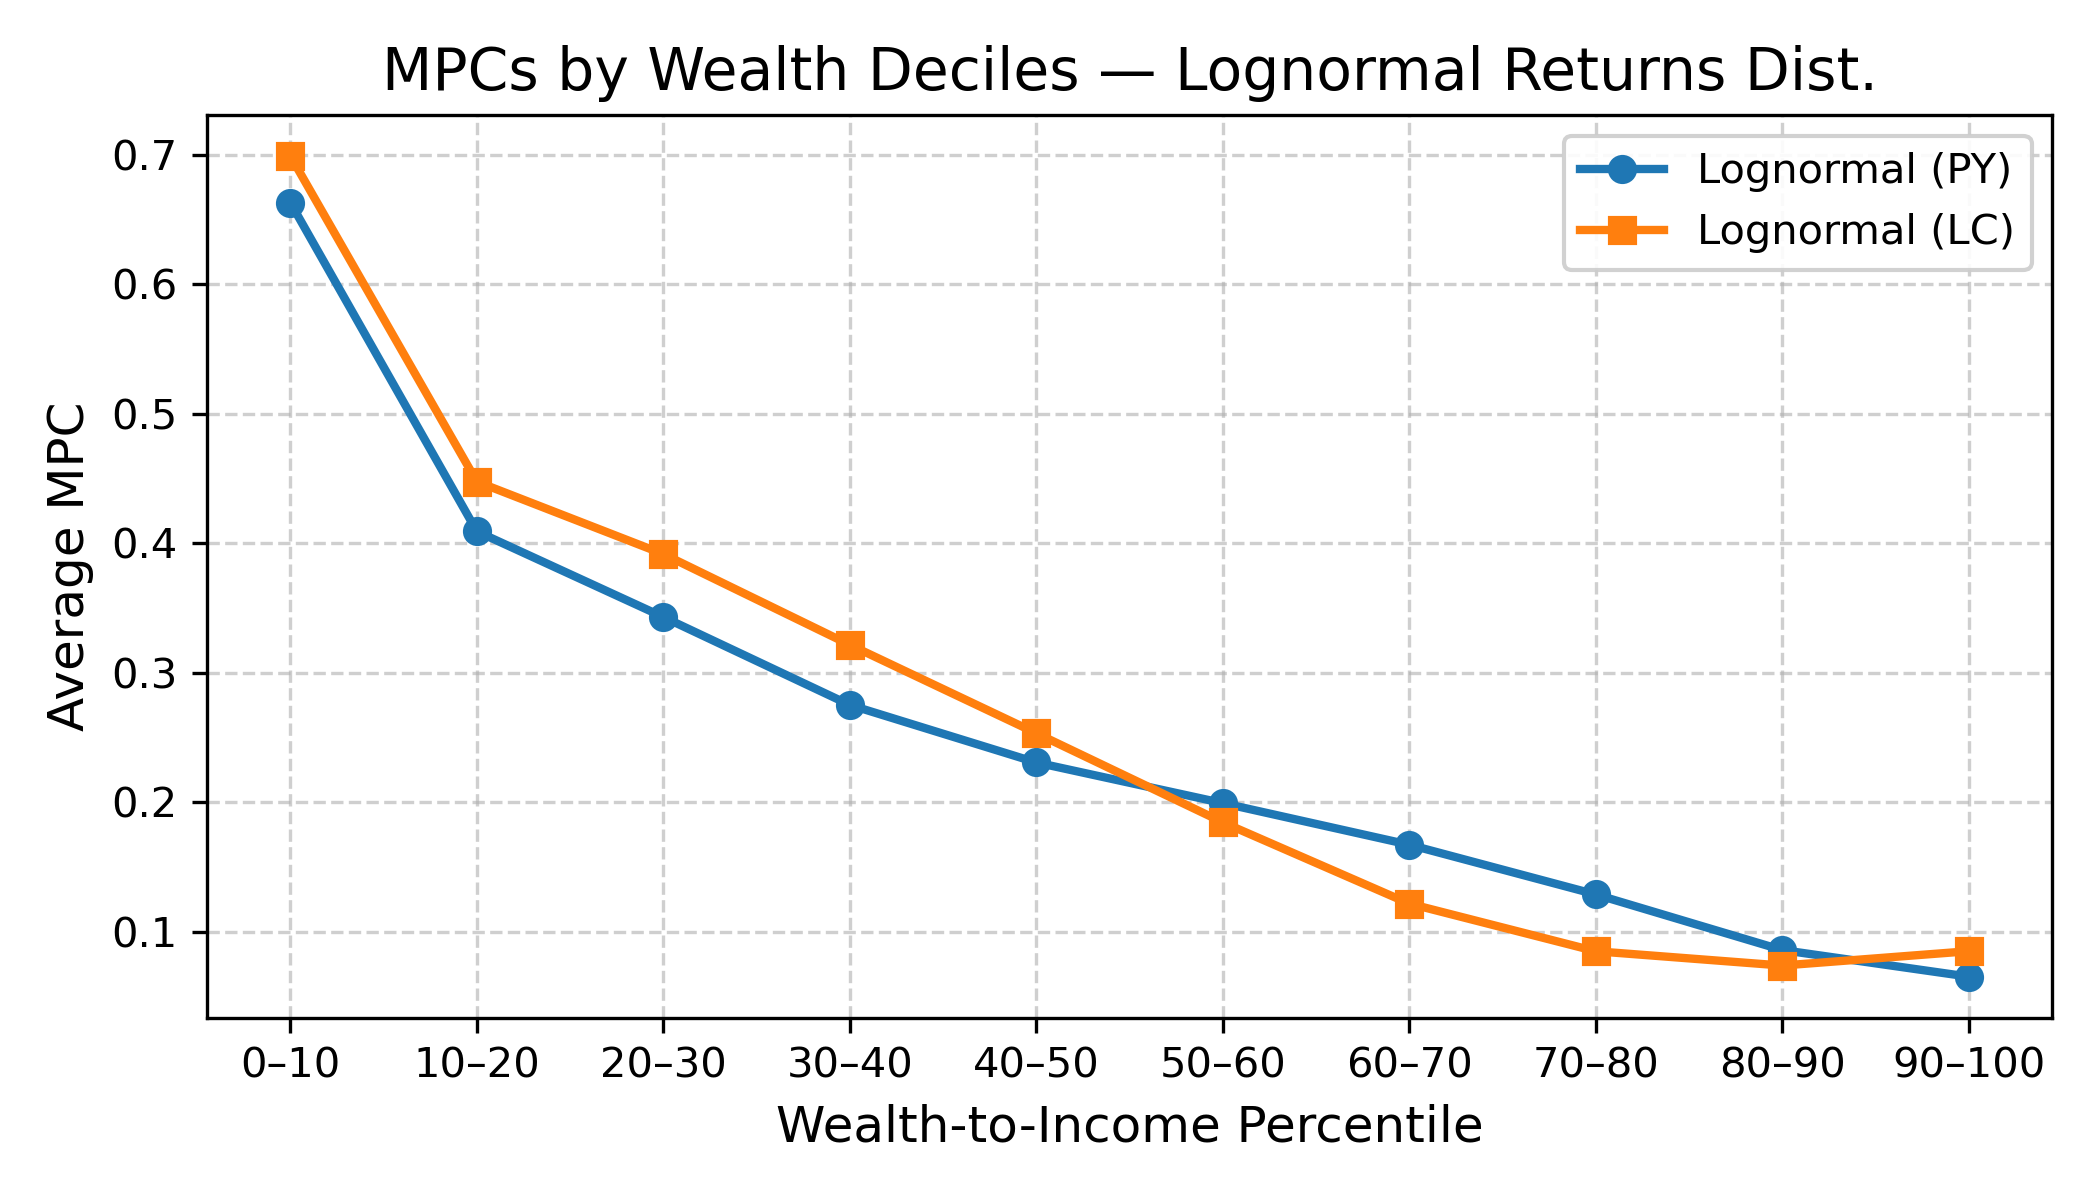
\includegraphics[width=0.8\textwidth]{Tables/Lognorm_PY_LC_MPC_by_WealthDecile_compare.png}
\label{fig:LognormPYLCMPCCompare}
\end{figure}


\par For the second set of untargeted moments, I include the cumulative wealth shares by age for this case of an estimated lognormal returns distribution. Again, these moments are closer to the empirical counterpart than the case with no heterogeneity. The best fits are for the wealth shares of older cohorts. 

\begin{figure}[h]
\centering
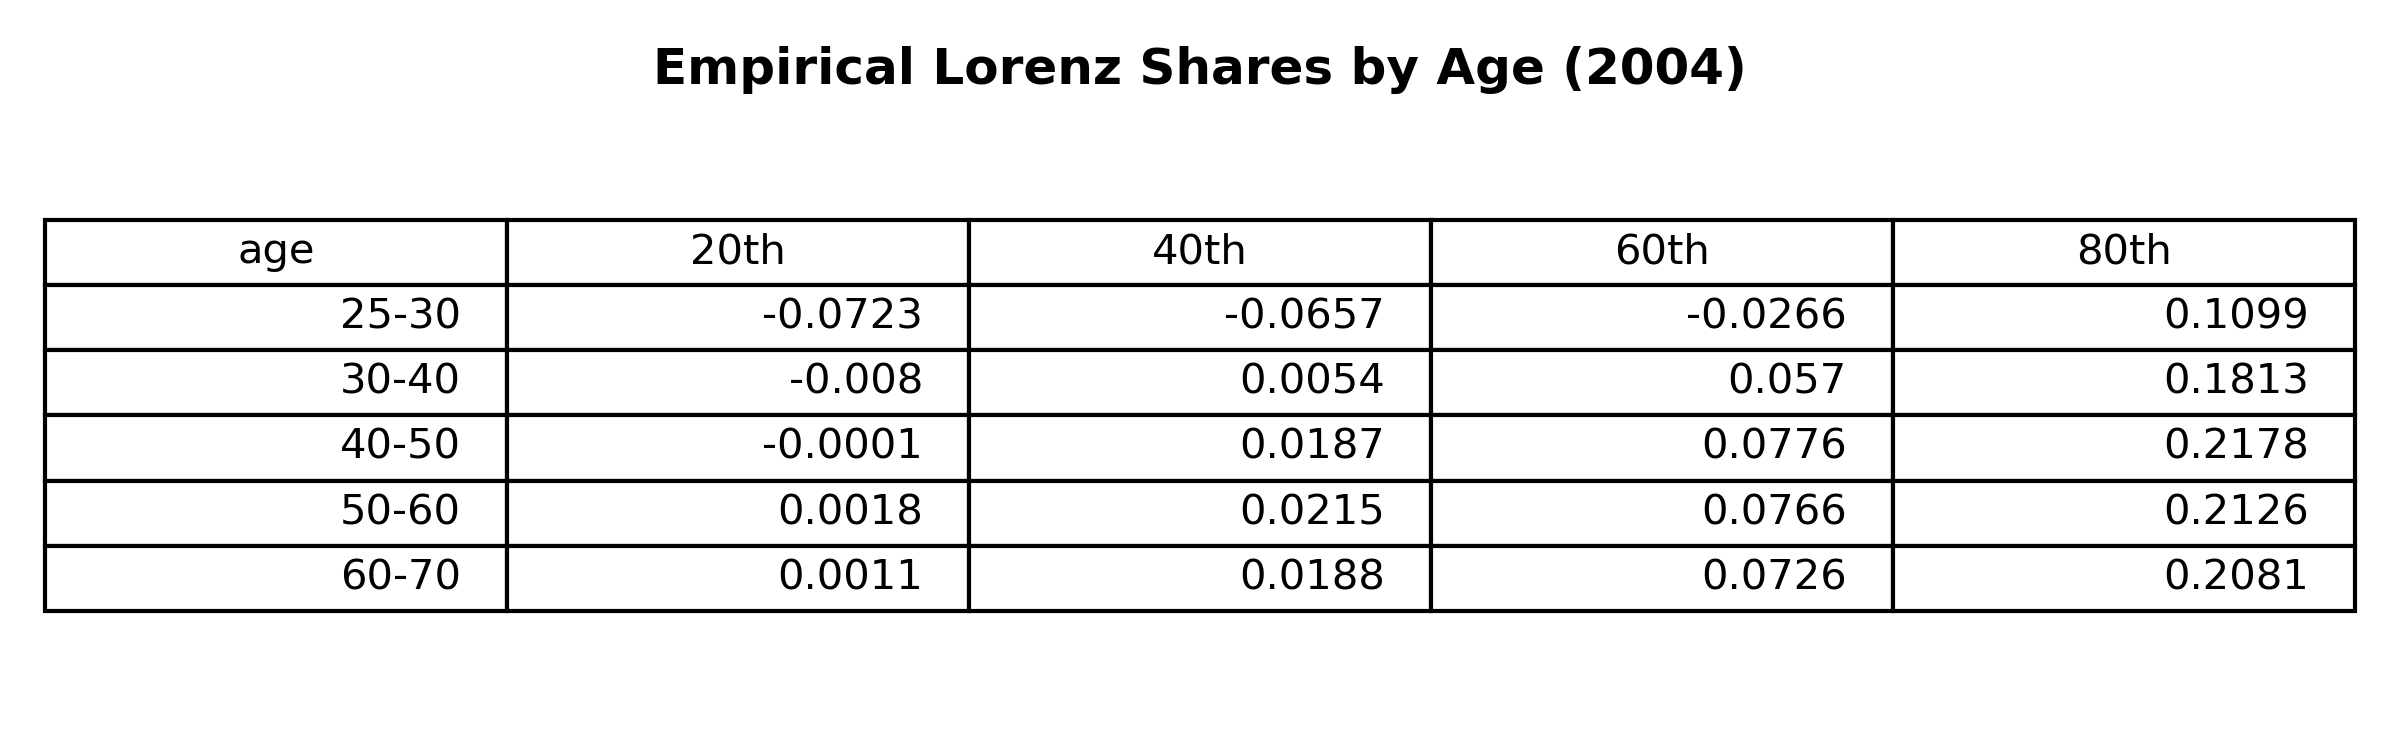
\includegraphics[width=0.8\textwidth]{Tables/Emp_Lorenz_by_age_2004.png}
\caption{Empirical Lorenz Curve Targets from the 2004 SCF.}
\label{fig:EmpLorenzTar}
\end{figure}

\begin{figure}[htbp]
\centering
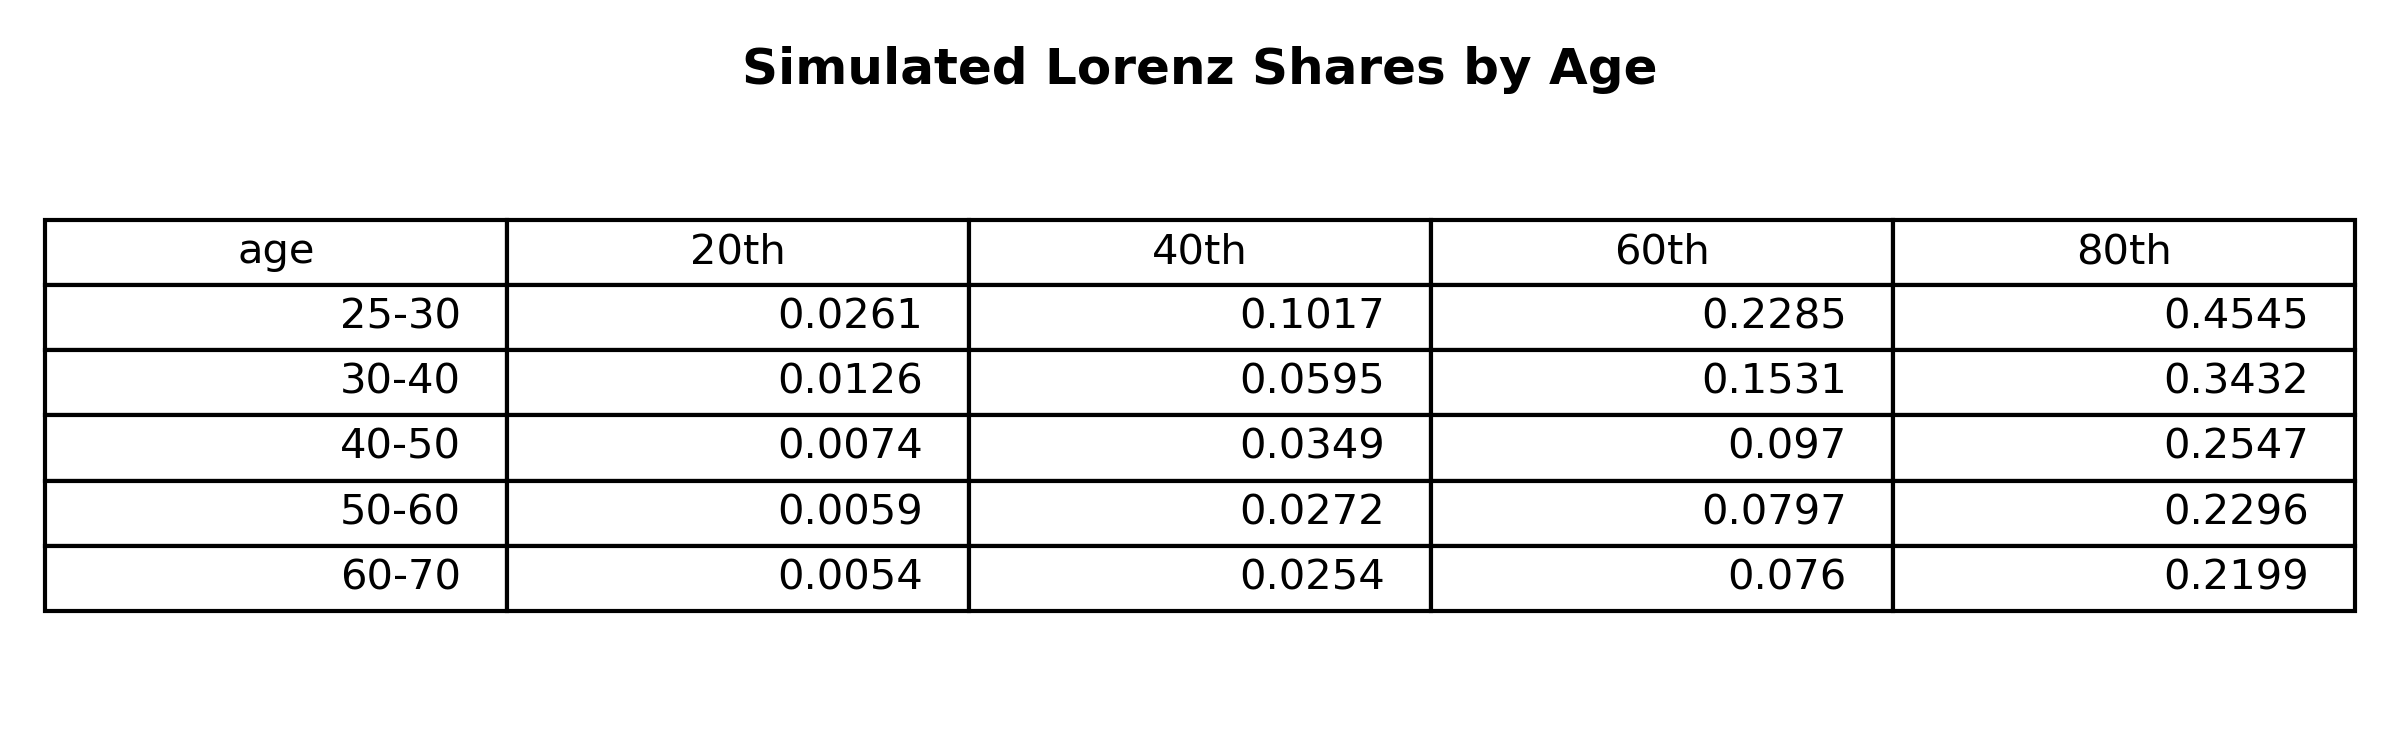
\includegraphics[width=0.8\textwidth]{Tables/Sim_Lorenz_by_age_Lognorm_LCrrDistNetWorth_2004.png}
\caption{Simulated Untargeted Moments with Heterogeneity (R-dist).}
\label{fig:SimLorenzTarDist}
\end{figure}

\subsection{Tax implications}

\par I also consider the tax implications of the model in this setting. I begin with comparing the effects of each of the tax policies on wealth inequality for both the infinite horizon and the life-cycle cases. The same relationship holds here: each effect of the tax is small (since the policies are revenue-equivalent and only raise $1\%$ of aggregate labor income), but the capital income tax reduces wealth inequality more.

% required in preamble:
% \usepackage{booktabs}
% \usepackage{graphicx}   % for \resizebox
% \usepackage{hyperref}   % for \hypertarget (optional if you already use it)

\hypertarget{taxPY_lognorm}{}
\begin{table}[H]
  \centering
  \resizebox{0.7\textwidth}{!}{%
    \begin{tabular}{@{} l c c c c @{}}
      \toprule
      \multicolumn{1}{c}{} & \multicolumn{4}{c}{Lorenz points} \\
      \midrule
      Tax scheme & 20\% & 40\% & 60\% & 80\% \\
      \midrule
      None & 0.60\% & 2.75\% & 7.27\% & 16.28\% \\[6pt]
      \shortstack[l]{Wealth \\$\tau_w = \text{0.34\%}$} & 0.67\% & 3.14\% & 8.38\% & 18.86\% \\[6pt]
      \shortstack[l]{Capital income \\$\tau_{ci} = \text{5.08\%}$} & 0.73\% & 3.37\% & 8.94\% & 20.02\% \\
      \bottomrule
    \end{tabular}%
  }
  \caption{Tax policies in the infinite horizon setting (lognormal returns across households).}
  \label{tab:taxPY_lognorm}
\end{table}
\unskip
% required in preamble:
% \usepackage{booktabs}
% \usepackage{graphicx}   % for \resizebox
% \usepackage{hyperref}   % for \hypertarget (optional if you already use it)

\hypertarget{taxLC_lognorm}{}
\begin{table}[H]
  \centering
  \resizebox{0.7\textwidth}{!}{%
    \begin{tabular}{@{} l c c c c @{}}
      \toprule
      \multicolumn{1}{c}{} & \multicolumn{4}{c}{Lorenz points} \\
      \midrule
      Tax scheme & 20\% & 40\% & 60\% & 80\% \\
      \midrule
      None & 0.42\% & 2.05\% & 5.98\% & 16.73\% \\[6pt]
      \shortstack[l]{Wealth \\$\tau_w = \text{0.33\%}$} 
            & 0.43\% & 2.12\% & 6.14\% & 16.86\% \\[6pt]
      \shortstack[l]{Capital income \\$\tau_{ci} = \text{4.97\%}$} 
            & 0.46\% & 2.23\% & 6.46\% & 17.72\% \\
      \bottomrule
    \end{tabular}%
  }
  \caption{Tax policies in the life-cycle setting (lognormal returns across households).}
  \label{tab:taxLC_lognorm}
\end{table}
\unskip

\par For the welfare effects in this setting, I begin with the expected welfare gains from starting with the wealth tax and switching to the capital income tax. Again, a newborn who didn't know their type would prefer the capital income tax over the wealth tax: the lifetime value of the newborn under the capital income regime is higher. 

\begin{table}[!htbp]
\centering
\caption{Expected Welfare Gains from Tax Reform (Lognormal Returns)}
\label{tab:ce_welfare_tax_lognorm}
\begin{threeparttable}
\begin{tabular}{lcc}
\toprule
& \textbf{Infinite horizon} & \textbf{Life-cycle} \\
\midrule
WT vs CIT       & 0.22\% & 0.18\% \\
WT vs Original  & 0.78\% & 0.36\% \\
CIT vs Original & 0.56\% & 0.18\% \\
\bottomrule
\end{tabular}
\begin{tablenotes}[flushleft]
\footnotesize
\item Notes: Entries are consumption-equivalent (CE) welfare gains, $\Delta$, expressed as percent changes under the assumption that individual returns follow a lognormal distribution across households. 
\end{tablenotes}
\end{threeparttable}
\end{table}


\par A decomposition of these welfare effects can be done by return type for the infinite horizon case, and by education-return type in the life-cycle scenario. The pattern of results remains the same, where only the highest type in each case prefers the wealth tax over the capital income tax. A notable difference between th distributional assumptions is that, the estimated lognormal distribution requires less types with returns less than 1 thanthe uniform distribution did. Despite this, the welfare results remain robust. 

% Requires: \usepackage{booktabs,threeparttable}
\begin{table}[!htbp]
\centering
\caption{Per-Type Welfare Gain and Baseline Return (WT vs CIT, Lognormal Returns)}
\label{tab:ce_per_type_wt_vs_cit_lognorm}
\begin{threeparttable}
\begin{tabular}{lccccccc}
\toprule
& \textbf{Type 1} & \textbf{Type 2} & \textbf{Type 3} & \textbf{Type 4} & \textbf{Type 5} & \textbf{Type 6} & \textbf{Type 7} \\
\midrule
Baseline $R$ (gross) & 0.976 & 1.001 & 1.014 & 1.026 & 1.038 & 1.053 & 1.079 \\
CE $\Delta$ (WT vs CIT, \%) & 0.267\% & 0.342\% & 0.329\% & 0.317\% & 0.308\% & 0.304\% & -0.326\% \\
\bottomrule
\end{tabular}
\begin{tablenotes}[flushleft]
\footnotesize
\item Notes: CE entries are per-type consumption-equivalent welfare gains (pmv-weighted within type), expressed as percent. Positive values favor the wealth tax over the capital income tax for that return type. Baseline $R$ values are pre-tax gross returns (low $\rightarrow$ high) under the lognormal returns specification.
\end{tablenotes}
\end{threeparttable}
\end{table}


% Requires: \usepackage{booktabs, threeparttable, multirow, graphicx}

\begin{table}[!htbp]
\centering
\caption{Per-Education Per-Type Welfare Gain and Baseline Return (WT vs CIT, Lognormal Returns)}
\label{tab:ce_per_type_wt_vs_cit_lc_lognorm}
\begin{threeparttable}

\begin{minipage}{\linewidth}
\centering
\resizebox{\linewidth}{!}{%
\begin{tabular}{llccccccc}
\toprule
\multicolumn{2}{c}{} & \textbf{Type 1} & \textbf{Type 2} & \textbf{Type 3} & \textbf{Type 4} & \textbf{Type 5} & \textbf{Type 6} & \textbf{Type 7} \\
\midrule
\multirow{2}{*}{NoHS}
  & Baseline $R$ (gross)        & 0.9363 & 0.9711 & 0.9910 & 1.0084 & 1.0260 & 1.0471 & 1.0865 \\
  & CE $\Delta$ (WT vs CIT, \%)  & 0.132\% & 0.176\% & 0.225\% & 0.275\% & 0.335\% & 0.292\% & -0.114\% \\
\midrule
\multirow{2}{*}{HS}
  & Baseline $R$ (gross)        & 0.9363 & 0.9711 & 0.9910 & 1.0084 & 1.0260 & 1.0471 & 1.0865 \\
  & CE $\Delta$ (WT vs CIT, \%)  & 0.131\% & 0.177\% & 0.229\% & 0.283\% & 0.332\% & 0.250\% & -0.098\% \\
\midrule
\multirow{2}{*}{College}
  & Baseline $R$ (gross)        & 0.9363 & 0.9711 & 0.9910 & 1.0084 & 1.0260 & 1.0471 & 1.0865 \\
  & CE $\Delta$ (WT vs CIT, \%)  & 0.131\% & 0.177\% & 0.228\% & 0.276\% & 0.311\% & 0.218\% & -0.096\% \\
\bottomrule
\end{tabular}%
} % end resizebox
\end{minipage}

\begin{tablenotes}[flushleft]
  \footnotesize
\item 
  Notes: CE entries are consumption-equivalent welfare gains (pmv-weighted within type), \\
  expressed as percent. Positive values favor wealth taxation over capital income taxation \\
  for that return type. Baseline $R$ are pre-tax gross returns by type (low $\rightarrow$ high)
  at $t=0$ \\ under the lognormal returns specification. 
\end{tablenotes}
\end{threeparttable}
\end{table}


\subsection{Mechanism for Bank Heterogeneity}

  \par To match each exercise that was done when the estimated distribution was Uniform, I include a table which captures the estimated returns distribution which best matches 2004 SCF data on net worth and the corresponding implied elasticities for both the infinte horizon and life-cycle settings here as well.  

  \begin{table}[!htbp]
\centering
\caption{Estimated Returns and Implied Elasticities (Lognormal)}
\label{tab:returns_lognormal}
\begin{tabular}{|c|c|c|c|}
\hline
\multicolumn{2}{|c|}{PY} & \multicolumn{2}{|c|}{LC} \\
\hline
Estimated returns & Implied elasticities & Estimated returns & Implied elasticities \\
\hline
0.976 & 8.231 & 0.936 & 5.898 \\
1.001 & 10.615 & 0.971 & 7.838 \\
1.014 & 12.602 & 0.991 & 9.532 \\
1.026 & 14.963 & 1.008 & 11.640 \\
1.038 & 18.366 & 1.026 & 14.874 \\
1.053 & 24.922 & 1.047 & 21.857 \\
1.079 & 68.242 & 1.086 & 127.378 \\
\hline
\end{tabular}
\end{table}
 